% -*- fill-column: 52 -*-
% (local-set-key (kbd "C-c C-f") 'display-fill-column-indicator-mode)
\chapter{Vezérlés}
\section{Rendezések}
Egy klasszikus -- és nagyon hasznos -- programozási
feladat számok listájának növekvő sorrendbe
rendezése. Erre rengeteg módszer van, itt csak a
legfontosabbak közül nézünk meg néhányat.

\subsection*{Beszúrásos rendezés}
Az első algoritmus a \emph{beszúrásos rendezés}. Az
ötlet a következő: ha van egy listám, akkor azt
szétszedem az első elemre és a maradékára, az
utóbbit (rekurzívan) rendezem, és végül az első
elemet beszúrom a ,,megfelelő'' helyre.
\index{rendezés!beszúrásos}
\begin{program}
rendez1([], []).
rendez1([X|M], Y) :-
    rendez1(M, M1), beszúr(X, M1, Y).
\end{program}
A megfelelő helyre való beszúrásnál pedig egyszerűen
addig megyünk, amíg egy legalább akkora elemet nem
találunk:
\begin{program}
beszúr(X, [], [X]).
beszúr(X, [Y|M], [X,Y|M]) :- X =< Y.
beszúr(X, [Y|M], [Y|M1]) :- X > Y, beszúr(X, M, M1).
\end{program}
Próbáljuk ki!
\begin{query}
?- rendez1([4,1,9,2,6,0,3,2,5,1], X).
X = [0, 1, 1, 2, 2, 3, 4, 5, 6, 9]
\end{query}

Ennek az algoritmusnak egy nagy előnye, hogy akkor
is jól használható, ha az adatokat folyamatosan
kapjuk, hiszen ha már van egy rendezett listánk,
akkor utána mindig elég a \pr{beszúr} műveletet
használni. Egy másik jó tulajdonsága, hogy egy már
rendezett sorozatnál nem végez plusz munkát, épp
csak ellenőrzi, hogy a lista tényleg jó sorrendben
van:
\begin{query}
?- trace, rendez1([1,2,3], X).
Call:rendez1([1, 2, 3], X)
  Call:rendez1([2, 3], X1)
    Call:rendez1([3], X2)
      Call:rendez1([], X3)
      Exit:rendez1([], [])
      Call:beszúr(3, [], X2)
      Exit:beszúr(3, [], [3])
    Exit:rendez1([3], [3])
    Call:beszúr(2, [3], X1)
      Call:2=<3
      Exit:2=<3
    Exit:beszúr(2, [3], [2, 3])
  Exit:rendez1([2, 3], [2, 3])
  Call:beszúr(1, [2, 3], X)
    Call:1=<2
    Exit:1=<2
  Exit:beszúr(1, [2, 3], [1, 2, 3])
Exit:rendez1([1, 2, 3], [1, 2, 3])
X = [1, 2, 3]
\end{query}

Ugyanakkor ha nincs szerencsénk, nem túl jó
hatásfokú: ha a lista $n$ hosszú, akkor kb.~$n^2$
összehasonlítást végez a legrosszabb esetben.

\subsection*{Gyorsrendezés}
A gyorsrendezésnél kiválasztunk egy tetszőleges
elemet (pl.~az elsőt), és a többit két részre
osztjuk aszerint, hogy nagyobb-e ennél vagy
sem. Ezután a két részt külön--külön rendezzük
(rekurzívan), majd az eredmény ezek összefűzéséből
adódik:
\index{rendezés!gyors}
\begin{program}
rendez2([], []).
rendez2([X|M], Y) :-
    szétoszt(X, M, Kicsi, Nagy),
    rendez2(Kicsi, K),
    rendez2(Nagy, N),
    hozzáfűz(K, [X|N], Y).
\end{program}
A szétosztás elég magától értetődő:
\begin{program}
szétoszt(_, [], [], []).
szétoszt(X, [Y|M], K, [Y|N]) :-
    X =< Y, szétoszt(X, M, K, N).
szétoszt(X, [Y|M], [Y|K], N) :-
    X > Y, szétoszt(X, M, K, N).
\end{program}

Ez (nagyon hosszú listákra) bizonyíthatóan sokkal
kevesebb ellenőrzést végez, mint a beszúrásos
rendezés. A fenti program azonban a hozzáfűzések
miatt nem igazán hatékony -- a következő leckében
majd szó lesz a különbség-listákról, amelyek
segítségével sokkal gyorsabbá tehető.

\subsection*{Fésülő rendezés}
Utolsónak nézzünk meg egy nagyon hasonló
algoritmust: itt is két részre bontjuk mindig a
listát, azokat rendezzük, majd összefűzzük, de itt
nem a szétválasztás a bonyolultabb, hanem az
összefűzés, vagy ez esetben az \emph{összefésülés}.
\index{rendezés!fésülő}

A listát a felénél kettéosztjuk, és mindkét részt
rendezzük (rekurzívan), végül a két rendezett listát
egy listává fésüljük össze:
\begin{program}
rendez3([], []).
rendez3([X], [X]).
rendez3(X, Y) :-
    kettéoszt(X, X1, X2),
    rendez3(X1, Y1),
    rendez3(X2, Y2),
    összefésül(Y1, Y2, Y).

kettéoszt([], [], []).
kettéoszt([X], [X], []).
kettéoszt([X,Y|M], [X|M1], [Y|M2]) :-
    kettéoszt(M, M1, M2).
\end{program}

Az összefésülésnél a két lista elemét
összehasonlítjuk, és a megfelelőt berakjuk a
maradékok összefűzéséből kapott listába:
\begin{program}
összefésül([X|Mx], [Y|My], [X|M]) :-
    X =< Y, összefésül(Mx, [Y|My], M).
összefésül([X|Mx], [Y|My], [Y|M]) :-
    X > Y, összefésül([X|Mx], My, M).
összefésül(X, [], X).
összefésül([], Y, Y).
\end{program}

Itt érdekes módon azt tapasztaljuk, hogy a (helyes)
eredményt végtelen sokszor megkapjuk. Ez azért van,
mert a \pr{rendez3} harmadik szabálya az egyelemű
listákra is meghívódhat. Ezt ki lehetne védeni
azzal, hogy megköveteljük, hogy legyen legalább két
eleme:
\begin{program}
rendez3(X, Y) :-
    X = [_,_|_], Y = [_,_|_],
    kettéoszt(X, X1, X2),
    rendez3(X1, Y1),
    rendez3(X2, Y2),
    összefésül(Y1, Y2, Y).
\end{program}
\dots de ez nem a legelegánsabb. (Hasonlóan, az
\pr{összefésül} utolsó két szabálya közt is van
átfedés.) Nincs valami jobb mód erre?

\begin{infobox*}{}{furcsa rendezések}
Rendezési algoritmusokból nincs hiány. Bizonyítható,
hogy a gyorsrendezés, a fésülő rendezés (és még sok
másik) a lehető leghatékonyabb\dots kivéve egy-két
furcsa módszert:
\begin{enumerate}
\item Vágjunk (száraz) spagettitésztákat az egyes
  számoknak megfelelő hosszokra, majd marokra fogva
  tegyük le az asztalra. Ezután egy kartonlapot
  rátéve mindig sorban vegyük ki azt, ami hozzáér a
  laphoz, és így egy csökkenő sorrendezéshez jutunk.
\item Vegyük a lista egy véletlenszerű
  permutációját, és ellenőrizzük, hogy sorban
  van-e. Ha igen, készen vagyunk. Ha nem, akkor
  robbantsuk fel a világot. Feltéve, hogy igaz a
  párhuzamos univerzumok elmélete, csak az az
  univerzum fog megmaradni, amelyikben a véletlen
  permutáció pont a helyes sorbarendezés volt.
\end{enumerate}
\index{rendezés!spagetti}\index{rendezés!véletlen}
\end{infobox*}      

\section{Vágás}
Egy szabály törzsében \emph{vágást} eszközölhetünk a
\pr{!} segítségével. Ez azt mondja, hogy ha már
idáig eljutottunk, akkor vagy sikerül teljesíteni a
törzs maradék részét, vagy ha nem, akkor úgy
vesszük, hogy ezzel a fejjel való egyesítés
sikertelen volt, nem próbálunk a \pr{!} előtti
kifejezésekre visszamenni, vagy az azonos fejhez
tartozó esetleges többi szabályt megnézni.
\index{vagas@vágás}\index{\pr{"!}}

Nézzük meg például az alábbi szabályokat, ahol
\pr{A}, \pr{B}, \pr{C} stb. kifejezéseket jelölnek:
\begin{program}
C :- P, Q, R, !, S, T, U.
C :- V.

A :- B, C, D.
\end{program}

Ekkor ha az
\begin{query}
?- A.
\end{query}
kérdést feltesszük, a következő fog történni:
\begin{enumerate}
\item Megnézi, hogy \pr{B} teljesül-e (tegyük fel,
  hogy igen).
\item Megnézi, hogy \pr{P}, \pr{Q}, \pr{R}
  teljesülnek-e (tegyük fel, hogy igen).
\item Megnézi, hogy \pr{S}, \pr{T}, \pr{U}
  teljesülnek-e. Tegyük fel, hogy az \pr{S} és
  \pr{T} teljesül, de az \pr{U} nem. Ekkor szokás
  szerint visszamegy a \pr{T}-re, és megkeresi annak
  egy másik megoldását stb.
\item Ha nem sikerült az \pr{S}, \pr{T}, \pr{U}-t
  teljesíteni, akkor -- a vágás miatt -- már nem
  megy vissza, hogy az \pr{R} egy másik megoldását
  keresse, és nem próbálkozik a \pr{C}-hez tartozó
  második szabállyal sem, hanem egy szinttel feljebb
  megy, és a \pr{B}-hez keres egy másik megoldást.
\end{enumerate}

\subsection*{Összefésülés hatékonyabban}
Nézzük meg, hogyan lehet ezzel feljavítani az összefésülést!
\begin{program}
összefésül([X|Mx], [Y|My], [X|M]) :-
    X =< Y, !, összefésül(Mx, [Y|My], M).
összefésül([X|Mx], [Y|My], [Y|M]) :-
    X > Y, !, összefésül([X|Mx], My, M).
összefésül(X, [], X) :- !.
összefésül([], Y, Y) :- !.
\end{program}

A vágások a programot hatékonyabbá teszik: ha az
első szabályban láttuk, hogy \pr{X =< Y}, már nem
kell ellenőrizni a többi szabályt stb. (Az utolsó
sorban a vágás felesleges, csak a szimmetria
kedvéért került bele.)

Hasonlóan, a \pr{rendez3} második szabályában:
\begin{program}
rendez3([X], [X]) :- !.
\end{program}
Ezekkel a módosításokkal már egyértelmű
(\emph{determinisztikus}) lesz a megoldás.
\index{determinisztikusság}

A vágások nem változtatják meg a program értelmét
(tehát, hogy milyen kifejezésekre lesz igaz), csak a
hatékonyságát.

\subsection*{Maximum}
Nézzünk egy másik példát! Az alábbi szabály két szám
közül kiválasztja a nagyobbikat:
\begin{program}
max1(X, Y, X) :- X >= Y.
max1(X, Y, Y) :- X < Y.
\end{program}
A fenti módon ez átírható így:
\begin{program}
max2(X, Y, X) :- X >= Y, !.
max2(X, Y, Y) :- X < Y.
\end{program}

Felmerül azonban ekkor, hogy a második szabályban szükség
van-e egyáltalán az \pr{X < Y} összehasonlításra,
hiszen csak akkor juthatunk oda, ha az \pr{X >= Y}
nem teljesült. A program akkor is működni látszik,
ha elhagyjuk:
\begin{program}
max3(X, Y, X) :- X >= Y, !.
max3(_, Y, Y).
\end{program}

Teszteljük egy kicsit!
\begin{query}
?- max3(3, 5, X).
X = 5
?- max3(4, 2, X).
X = 4
?- max3(1, 5, 5).
true
?- max3(5, 1, 1). % Ajjaj...
true
\end{query}

Hoppá! Mi történt?  Mivel az utolsó példában
mindhárom argumentumnak van értéke, és az első és
harmadik nem azonos, az első szabállyal nem is
próbálkozik, hanem rögtön a másodikra megy, ami
pedig most, hogy kivettük a feltételt, teljesül.

A \pr{max3} változatban megváltozott a program
deklaratív jelentése, hiszen egy olyan tényt
tartalmaz, ami magában nézve nem igaz. Ez általában
kerülendő, bár a hatékonysághoz néha szükséges. Ha
ilyen gondolatmenetet alkalmazunk, nagyon óvatosnak
kell lenni -- itt pl. biztosnak kell lennünk benne,
hogy a harmadik argumentum mindig változó.

\subsection*{Hozzáadás halmazhoz}
Egy további példaként nézzük meg az alábbi szabályt:

\begin{program}
% hozzáad(+X, +Halmaz, -Eredmény).
% Hozzáadja X-et a Halmaz listához,
% de csak akkor, ha az még nem tartalmazta.
hozzáad(X, L, L) :- tartalmaz(X, L), !.
hozzáad(X, L, [X|L]).
\end{program}

A vágás nélkül itt a második szabályt nehezebb lenne
megfogalmazni, kéne hozzá a 3. leckéhez tartozó
projektben látott \pr{nemtartalmaz} szabály, és
következésképp a hatékonyságból is vesztene.

Cserébe itt is problémába ütközünk, ha a harmadik
argumentum nem változó:
\begin{query}
?- hozzáad(b, [a,b], [b,a,b]).
true
\end{query}
Ezt elkerülendő, érdemes a dokumentációval\index{dokumentáció}
egyértelművé tenni a használatot. A fenti programhoz
tartozó megjegyzés is ilyen szellemben íródott. Az
első sorában egy egyezményes jelölésrendszert
használ, melyben minden argumentum háromféle lehet:
\begin{itemize}
\item \pr{+X} : kell, hogy legyen értéke
\item \pr{?X} : lehet értéke, de nem muszáj
\item \pr{-X} : csak változó lehet
\end{itemize}
Például:
\begin{enumerate}
\item \pr{+X > +Y} [4.~lecke]
\item \pr{lapít(+Eredeti, -Lapos)} [3.~lecke]
\item \pr{tartalmaz(?Elem, ?Lista)} [3.~lecke]
\end{enumerate}
Az első esetben mindkét kifejezésnek ismertnek kell
lennie; a másodikban a lapítandó lista ismert, és a
lapított verzió csak változó lehet; a harmadikban
pedig mind a lista, mind a benne tartalmazandó elem
lehet változó vagy ismert is.

\begin{problem}
Nézzük meg az alábbi szabályokat!
\begin{program}
p(1).
p(2) :- !.
p(3).
\end{program}       
Mit lesz az összes válasz az alábbi kérdésekre:
\begin{query}
?- p(X).
?- p(X), p(Y).
?- p(X), !, p(Y).
\end{query}
\end{problem}
\begin{problem}
Írd át hatékonyabbra a \pr{szétoszt} szabályt
vágások segítségével!
\end{problem}

\section{Tagadás}
Hogyan tudjuk megfogalmazni azt, hogy ,,Csilla
szeret minden állatot, kivéve a pókokat''?
\begin{program}
szereti(csilla, X) :- pók(X), !, fail.
szereti(csilla, X) :- állat(X).
\end{program}
(Általában ilyenkor a \pr{false} helyett a
\pr{fail}-t szokás használni, de a kettő jelentése
azonos.)\index{\pr{fail}}\index{tagadás}

Próbáljuk ki!
\begin{program}
állat(tarantula).
állat(denevér).
pók(tarantula).
\end{program}
\begin{query}
?- szereti(csilla, tarantula).
false
?- szereti(csilla, denevér).
true
\end{query}
Ez annyira hasznos, hogy érdemes bevezetni, mint
tagadást:
\begin{program}
nem(P) :- P, !, fail.
nem(_).
\end{program}

Figyeljük meg, hogy itt valami olyat csináltunk,
amit eddig még soha: egy változót (\pr{P}) a
törzsben magában használtunk. Ez feltételezi, hogy a
\pr{P}-nek kiszámolható az igazságértéke. Például a
fenti példát átírva:
\begin{program}
szereti(csilla, X) :- állat(X), nem(pók(X)).
\end{program}
Itt a \pr{P} értéke a \pr{pók(X)} struktúra, és a
\pr{nem} törzsében levő \pr{P} kiértékelésekor ezt
mint megoldandó célkifejezést értelmezi.

\subsection*{A ,,zárt világ'' feltétel}
A tagadásnak ez a módja nem mindig intuitív. Egy így
tagadott kifejezés akkor lesz igaz, ha a kifejezés
nem bizonyítható.\index{zart@zárt világ}

Mi történik, ha az előző programban felcseréljük a
törzs két tagját?
\begin{program}
szereti(csilla, X) :- nem(pók(X)), állat(X).
\end{program}
Érdekes módon Csilla most már a denevéreket sem
szereti! Miért? Azért, mert a \pr{nem(pók(X))}-ben
az \pr{X} egy változó, tehát a \pr{pók(X)}
bizonyítható az \pr{X = tarantula} helyettesítéssel,
így a \pr{nem(pók(X))} nem teljesül. Az érték
nélküli argumentumokkal tehát vigyázni kell.

Hasonlóan furcsa lehet, hogy
\begin{query}
?- nem(állat(kutya)).
true
\end{query}
\dots de persze helyes, hiszen a programban levő
szabályok alapján nem bizonyítható, hogy a kutya
állat.

Ezek miatt a \pr{nem} (vagy az angol \pr{not})
helyett a \pr{\textbackslash+} operátort szokás
használni, melynek definíciója ugyanaz, csak az
elnevezés kevésbé félrevezető:
\begin{program}
szereti(csilla, X) :- állat(X), \+ pók(X).
\end{program}
\index{\pr{\textbackslash+}}

\begin{problem}
Milyen kérdéssel lehet a \pr{Jelöltek} listából
kiválasztani azokat, akik nem szerepelnek a
\pr{Kiesettek} listában? Használjátok a
\pr{tartalmaz} szabályt és a tagadást!
\end{problem}
\begin{problem}
Készítsetek szabályt, ami két halmaz különbségét
képzi! (A halmaz itt egy olyan lista, amiben minden
elem egyszer fordul elő.)
\begin{query}
?- különbség([a,b,c,d], [f,d,b,e], X).
X = [a, c]
\end{query}
\end{problem}
\begin{problem}
Készítsetek szabályt, ami kiválogatja egy listából
azokat a kifejezéseket, amelyek egy adott másik
kifejezéssel egyesíthetőek!
\begin{query}
?- egyesíthető([X,b,t(Y)], t(a), L).
L = [X, t(Y)]
\end{query}
Figyeljetek arra, hogy az \pr{X} és \pr{Y} ne kapjon
ezáltal értéket!
\end{problem}

\section{Projekt: Katamino}
Készítsünk megoldót a Katamino-feladványokhoz!

\begin{center}
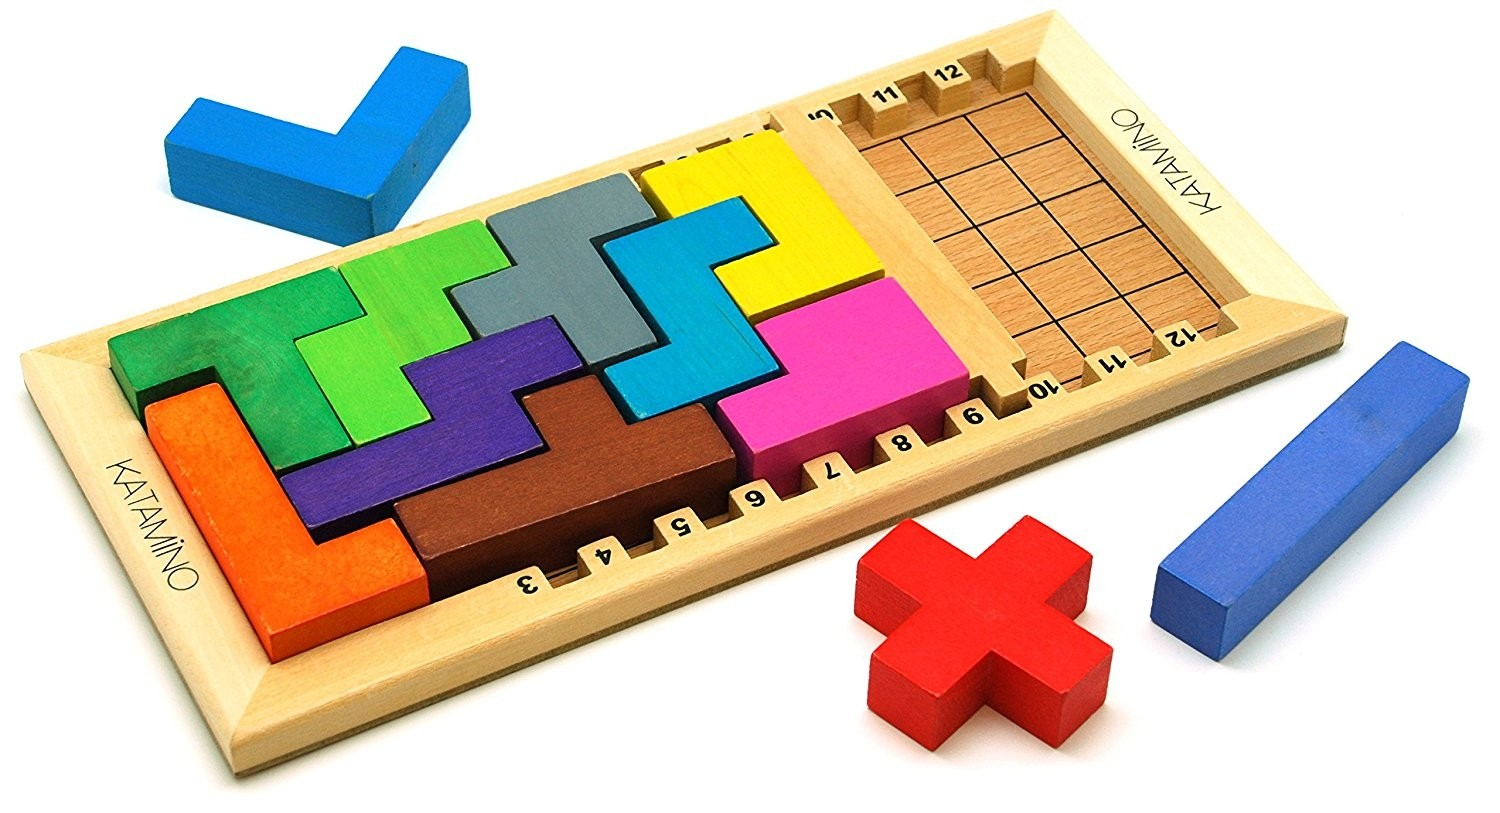
\includegraphics[width=\textwidth]{images/katamino.jpg}
\end{center}

A feladat mindig az, hogy a 12 pentominó egy adott
részhalmazából rakjunk ki egy $5\times n$-es
téglalapot.

\subsection*{Reprezentáció}
Az első lépés továbbra is az, hogy valahogyan le
kell írni a gép számára az adatokat, vagyis a
használható alakzatokat. Sokféle leírás
elképzelhető; itt most csináljuk a következőt:
minden egyes alakzatot a körülírható téglalap bal
alsó sarkához képest számolt koordinátáival írjuk
le.

Például a T-alakzatnál:
\begin{center}
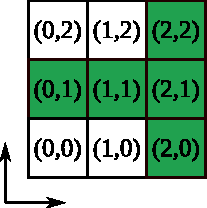
\includegraphics[width=.3\textwidth]{images/pentomino.pdf}
\end{center}
Ha a bal alsó sarok a $(0,0)$ pont, akkor az
alakzathoz tartozó pontok a következők: $(0,1)$,
$(1,1)$, $(2,0)$, $(2,1)$ és $(2,2)$. A pontokat
$x$-koordináta szerint, és azon belül $y$-koordináta
szerint rendezve írjuk fel.

Az $x$ és $y$-koordináták összefogására bármilyen
struktúrát használhatunk, pl. \pr{p(0,1)}, de a
tömörség kedvéért szokás a \pr{-} operátort
alkalmazni: \pr{0-1}. Bár az egyes
forgatások/tükrözések programból is legenerálhatóak,
egyszerűbb mindegyiket külön adatként megadni.

A T esetében pl.:
\begin{program}
alakzat(t, [0-0,0-1,0-2,1-1,2-1]).
alakzat(t, [0-0,1-0,1-1,1-2,2-0]).
alakzat(t, [0-1,1-1,2-0,2-1,2-2]).
alakzat(t, [0-2,1-0,1-1,1-2,2-2]).
\end{program}

Hasonlóan lehet definiálni a többi alakzatot,
amelyek mind valamilyen 1 betűből álló kódot kaptak:
\pr{k}, \pr{p}, \pr{c} stb. (Az összes alakzat, a
teljes program forráskódjával együtt, a lecke végén
található.)

\subsection*{Megoldó}
A programunk fő szabálya a \pr{kirak} lesz, ami egy
alakzat-listához megadja, hogy hogyan fog kinézni a
tábla. A megoldás módszere nagyon egyszerű: mindig a
(balról/alulról) első lyukat próbáljuk betömni.

\begin{program}
kirak(Ak, X) :- hossz(Ak, N), kirak(Ak, N, [], X).

kirak([], _, T, T).
kirak(Ak, N, T, X) :-
    első_lyuk(N, T, P),
    töröl(A, Ak, Ak1),
    letesz(A, P, N, T, T1),
    kirak(Ak1, N, T1, X).
\end{program}
A 2-argumentumú változat megnézi, hogy hány
alakzatot kapott (tehát milyen hosszú a tábla), és
meghívja a 4-argumentumú testvérét. Ez a
felhasználható alakzatokon (\pr{Ak}) kívül még
megkapja a tábla hosszát (\pr{N}), a tábla jelenlegi
állapotát (\pr{T}), és ezáltal kiszámolja a
kitöltött táblát (\pr{X}).

Ehhez megkeresi az első lyukat, majd kiválaszt
(töröl) egy alakzatot, azt leteszi úgy, hogy lefedje
a lyukat, és rekurzívan folytatja a műveletet, amíg
mindent le nem rak.

A tábla állapotát egy listában tároljuk, aminek az
elemei \pr{h(X-Y,A)} alakban adják meg, hogy az
\pr{X-Y} pozíción az \pr{A} alakzat egy darabja
található. Az első lyuk megkeresése így nagyon
egyszerű:
\begin{program}
első_lyuk(N, T, X-Y) :-
    között(1, N, X), között(1, 5, Y),
    \+ tartalmaz(h(X-Y,_), T), !.
\end{program}

Visszatérve az \pr{első\_lyuk}-ra, ez deklaratív
olvasatban azt mondja, hogy az \pr{X-Y} koordináták
a megfelelő keretek között vannak, és a tábla ezen a
pozíción nem tartalmaz elemet. Mitől fogja ez az
elsőt adni? Azért, mert a procedurális olvasatból
tudjuk, hogy sorban fog próbálkozni, tehát először
az \pr{X = 1} eseteket próbálja végig különböző
\pr{Y} értékekre, aztán az \pr{X = 2}-t stb., és a
végén levő vágásnak köszönhetően nem fog további
lyukakat megadni akkor sem, ha a keresés visszalépne
ide.

Már csak a \pr{letesz(A, X-Y, N, T, T1)} szabály van
hátra. Ez megpróbálja az \pr{A} alakzatot lerakni
úgy, hogy lefedje az \pr{X-Y} pontot, ne menjen ki
az $5\times n$-es táblából, és ne takarjon olyan
pozíciókat, amelyek szerepelnek \pr{T}-ben. Ha
sikerül, akkor az alakzat lehelyezésével kapott új
tábla a \pr{T1}.
\begin{program}
letesz(A, X-Y, N, T, T1) :-
    alakzat(A, [_-Dy|Dk]),
    Y1 is Y - Dy, Y1 > 0,
    letesz(A, X-Y1, Dk, N, [h(X-Y,A)|T], T1).
\end{program}
Ez tehát az \pr{A} alakzatnak kiválasztja egy
forgatását, és megnézi az első pontjának az
$y$-koordinátáját (\pr{Dy}). Az \pr{Y} koordinátánál
ennyivel lejjebb kell rakni az alakzatot, hogy az
első pont fedje a lyukat (hiszen az első pont az
alakzat legbaloldalibb, és azon belül legalsó
pontja). Ha ez a módosult \pr{Y1} koordináta nem
pozitív, akkor az alakzat kilóg.

A tényleges lerakási kísérletet a \pr{letesz}
6-argumentumú változata végzi:
\begin{program}
letesz(_, _, [], _, T, T).
letesz(A, X-Y, [Dx-Dy|Dk], N, T, T1) :-
    X1 is X + Dx, között(1, N, X1),
    Y1 is Y + Dy, között(1, 5, Y1),
    \+ tartalmaz(h(X1-Y1,_), T),
    letesz(A, X-Y, Dk, N, [h(X1-Y1,A)|T], T1).
\end{program}
Ez plusz argumentumként megkapja a kiválasztott
forgatáshoz tartozó pontokat is (az első kivételéve,
amivel a lyukat fedtük), és ezeken megy végig
rekurzívan. Minden lépésben a (módosított) \pr{X-Y}
koordináta alapján kiszámolja, hogy hova kerül a
pont, és ellenőrzi, hogy értelmes-e a koordináta és
nincs-e már lefedve \pr{T}-ben.

\subsection*{Kiíratás}
A lényeggel ugyan már készen vagyunk, de az eredmény
nehezen olvasható:
\begin{query}
?- kirak([l,t,w,k,y,r,z,c,p], X).
  X = [h(9-5, c), h(9-4, c), h(9-3, c), h(8-5, c),
       h(8-3, c), h(9-2, p), h(9-1, p), h(8-2, p),
       h(8-1, p), h(7-1, p), h(8-4, z), h(7-4, z),
       h(7-3, z), h(7-2, z), h(6-2, z), h(7-5, r),
       h(6-5, r), h(6-4, r), h(6-3, r), h(5-4, r),
       h(5-5, w), h(4-5, w), h(4-4, w), h(3-4, w),
       h(3-3, w), h(6-1, y), h(5-2, y), h(5-1, y),
       h(4-1, y), h(3-1, y), h(5-3, k), h(4-3, k),
       h(4-2, k), h(3-2, k), h(2-2, k), h(3-5, t),
       h(2-5, t), h(2-4, t), h(2-3, t), h(1-5, t), 
       h(2-1, l), h(1-4, l), h(1-3, l), h(1-2, l),
       h(1-1, l)]
\end{query}

Próbáljuk meg kiíratni egy kicsit ,,grafikusabb''
formában! Az elsődleges szabályunk akkor ez lesz:
\begin{program}
katamino(Ak) :-
    hossz(Ak, N), kirak(Ak, X), kiír(N, X).
\end{program}

A \pr{kiír(N, T)} pedig 5 sorba rendezve szépen
kiírja az \pr{N} hosszú \pr{T} táblát. A kiíráshoz a
\pr{write(X)} kifejezést fogjuk használni, ami
kiírja az \pr{X} értékét, új sor nyitásához pedig a
\pr{nl}-t (\emph{newline}, újsor).
\index{\pr{write}}\index{\pr{nl}}
\begin{program}
kiír(N, T) :- kiír(N, 1-5, T).

kiír(_, _-0, _).
kiír(N, X-Y, T) :-
    Y =< 5, X > N, Y1 is Y - 1,
    nl, kiír(N, 1-Y1, T).
kiír(N, X-Y, T) :-
    Y =< 5, X =< N,
    tartalmaz(h(X-Y,A), T),
    write(A), write(' '),
    X1 is X + 1,
    kiír(N, X1-Y, T).
\end{program}
A 2-argumentumú változat csak átadja a feladatot a
3-argumentumúnak, ami megkapja az éppen kiírandó
elem \pr{X-Y} koordinátáját is. Ennek három szabálya
van:
\begin{enumerate}
\item Ha már a 0. sort kéne kiírni, készen vagyunk.
\item Ha \pr{X > N}, akkor vége az aktuális sornak,
  új sort kezdünk. Az \pr{Y} koordináta felülről
  megy lefelé, mert a kiírás is felülről lefelé
  történik.
\item Egyébként megkeresi, hogy az \pr{X-Y} pozíción
  melyik alakzat található, és kiírja, utána kiír
  még egy szóközt, és továbbmegy a következő \pr{X}
  pozícióra.
\end{enumerate}
Nézzük meg!
\begin{query}
?- katamino([l,t,w,k,y,r,z,c,p]).
t t t w w r r c c 
l t w w r r z z c 
l t w k k r z c c 
l k k k y z z p p 
l l y y y y p p p 
true
\end{query}
És ez éppen az a megoldás, ami a képen van! Erre
persze elég jó esély volt, ugyanis a felhasználandó
alakzatok listáját hozzávetőlegesen a képen látható
megoldás sorrendjében adtuk meg. Egy másik
permutáció más megoldást talál meg először:
\begin{query}
?- katamino([t,w,l,k,r,z,y,p,c]).
w y y y y l l l l 
w w y p p p r r l 
t w w p p z z r r 
t t t k k z c r c 
t k k k z z c c c 
true 
\end{query}

\begin{problem}
A Katamino szabályai szerint a kirakandó téglalap
magassága mindig 5. Oldjuk fel ezt a korlátot!
Írjátok át a programot úgy, hogy a \pr{katamino}
szabály paraméterben kapja meg a magasságot is, és
ennek megfelelő megoldást keressen! A program vegye
észre rögtön, ha a magasság nem illik a megkapott
alakzatok számához (pl.~10 alakzat és 7-es
magasság). Keressetek megoldást a $3\times20$,
$4\times15$, $5\times12$, $6\times10$ téglalapok
kitöltésére! (Tipp: a szabályokban az eddigi \pr{N}
paramétert cseréljétek \pr{N-M} párra.)
\end{problem}

\subsection*{A teljes program}
\begin{program}
katamino(Ak) :-
    hossz(Ak, N), kirak(Ak, X), kiír(N, X).

% Megoldó

kirak(Ak, X) :- hossz(Ak, N), kirak(Ak, N, [], X).

kirak([], _, T, T).
kirak(Ak, N, T, X) :-
    első_lyuk(N, T, P),
    töröl(A, Ak, Ak1),
    letesz(A, P, N, T, T1),
    kirak(Ak1, N, T1, X).

első_lyuk(N, T, X-Y) :-
    között(1, N, X), között(1, 5, Y),
    \+ tartalmaz(h(X-Y,_), T), !.

letesz(A, X-Y, N, T, T1) :-
    alakzat(A, [_-Dy|Dk]),
    Y1 is Y - Dy, Y1 > 0,
    letesz(A, X-Y1, Dk, N, [h(X-Y,A)|T], T1).

letesz(_, _, [], _, T, T).
letesz(A, X-Y, [Dx-Dy|Dk], N, T, T1) :-
    X1 is X + Dx, között(1, N, X1),
    Y1 is Y + Dy, között(1, 5, Y1),
    \+ tartalmaz(h(X1-Y1,_), T),
    letesz(A, X-Y, Dk, N, [h(X1-Y1,A)|T], T1).

% Kiírás

kiír(N, T) :- kiír(N, 1-5, T).

kiír(_, _-0, _).
kiír(N, X-Y, T) :-
    Y =< 5, X > N, Y1 is Y - 1,
    nl, kiír(N, 1-Y1, T).
kiír(N, X-Y, T) :-
    Y =< 5, X =< N,
    tartalmaz(h(X-Y,A), T),
    write(A), write(' '),
    X1 is X + 1,
    kiír(N, X1-Y, T).

% Segéd-szabályok

tartalmaz(X, [X|_]).
tartalmaz(X, [_|Maradék]) :- tartalmaz(X, Maradék).

töröl(X, [X|M], M).
töröl(X, [Y|M], [Y|M1]) :- töröl(X, M, M1).

hossz([], 0).
hossz([_|M], N) :- hossz(M, N1), N is 1 + N1.

között(N, M, N) :- N =< M.
között(N, M, X) :-
    N < M, N1 is N + 1,
    között(N1, M, X).

% Alakzatok

% kígyó (lila)
alakzat(k, [0-0,0-1,0-2,1-2,1-3]).
alakzat(k, [0-0,0-1,1-1,1-2,1-3]).
alakzat(k, [0-0,1-0,1-1,2-1,3-1]).
alakzat(k, [0-0,1-0,2-0,2-1,3-1]).
alakzat(k, [0-1,0-2,0-3,1-0,1-1]).
alakzat(k, [0-1,1-0,1-1,2-0,3-0]).
alakzat(k, [0-1,1-1,2-0,2-1,3-0]).
alakzat(k, [0-2,0-3,1-0,1-1,1-2]).
% P-betű (rózsaszín)
alakzat(p, [0-0,0-1,0-2,1-0,1-1]).
alakzat(p, [0-0,0-1,0-2,1-1,1-2]).
alakzat(p, [0-0,0-1,1-0,1-1,1-2]).
alakzat(p, [0-0,0-1,1-0,1-1,2-0]).
alakzat(p, [0-0,0-1,1-0,1-1,2-1]).
alakzat(p, [0-0,1-0,1-1,2-0,2-1]).
alakzat(p, [0-1,0-2,1-0,1-1,1-2]).
alakzat(p, [0-1,1-0,1-1,2-0,2-1]).
% C-betű (sárga)
alakzat(c, [0-0,0-1,0-2,1-0,1-2]).
alakzat(c, [0-0,0-1,1-0,2-0,2-1]).
alakzat(c, [0-0,0-1,1-1,2-0,2-1]).
alakzat(c, [0-0,0-2,1-0,1-1,1-2]).
% W-betű (világoszöld)
alakzat(w, [0-0,0-1,1-1,1-2,2-2]).
alakzat(w, [0-0,1-0,1-1,2-1,2-2]).
alakzat(w, [0-1,0-2,1-0,1-1,2-0]).
alakzat(w, [0-2,1-1,1-2,2-0,2-1]).
% L-betű (narancssárga)
alakzat(l, [0-0,0-1,0-2,0-3,1-0]).
alakzat(l, [0-0,0-1,0-2,0-3,1-3]).
alakzat(l, [0-0,0-1,1-0,2-0,3-0]).
alakzat(l, [0-0,0-1,1-1,2-1,3-1]).
alakzat(l, [0-0,1-0,1-1,1-2,1-3]).
alakzat(l, [0-0,1-0,2-0,3-0,3-1]).
alakzat(l, [0-1,1-1,2-1,3-0,3-1]).
alakzat(l, [0-3,1-0,1-1,1-2,1-3]).
% Y-betű vagy tengeralattjáró (barna)
alakzat(y, [0-0,0-1,0-2,0-3,1-1]).
alakzat(y, [0-0,0-1,0-2,0-3,1-2]).
alakzat(y, [0-0,1-0,1-1,2-0,3-0]).
alakzat(y, [0-0,1-0,2-0,2-1,3-0]).
alakzat(y, [0-1,1-0,1-1,1-2,1-3]).
alakzat(y, [0-1,1-0,1-1,2-1,3-1]).
alakzat(y, [0-1,1-1,2-0,2-1,3-1]).
alakzat(y, [0-2,1-0,1-1,1-2,1-3]).
% I-betű vagy egyenes (kék)
alakzat(i, [0-0,0-1,0-2,0-3,0-4]).
alakzat(i, [0-0,1-0,2-0,3-0,4-0]).
% r-betű (szürke)
alakzat(r, [0-0,0-1,1-1,1-2,2-1]).
alakzat(r, [0-0,1-0,1-1,1-2,2-1]).
alakzat(r, [0-1,0-2,1-0,1-1,2-1]).
alakzat(r, [0-1,1-0,1-1,1-2,2-0]).
alakzat(r, [0-1,1-0,1-1,1-2,2-2]).
alakzat(r, [0-1,1-0,1-1,2-1,2-2]).
alakzat(r, [0-1,1-1,1-2,2-0,2-1]).
alakzat(r, [0-2,1-0,1-1,1-2,2-1]).
% V-betű vagy sarok (kék)
alakzat(v, [0-0,0-1,0-2,1-0,2-0]).
alakzat(v, [0-0,0-1,0-2,1-2,2-2]).
alakzat(v, [0-0,1-0,2-0,2-1,2-2]).
alakzat(v, [0-2,1-2,2-0,2-1,2-2]).
% Z-betű vagy S-betű (kék)
alakzat(z, [0-0,0-1,1-1,2-1,2-2]).
alakzat(z, [0-0,1-0,1-1,1-2,2-2]).
alakzat(z, [0-1,0-2,1-1,2-0,2-1]).
alakzat(z, [0-2,1-0,1-1,1-2,2-0]).
% pluszjel (piros)
alakzat(+, [0-1,1-0,1-1,1-2,2-1]).
% T-betű (zöld)
alakzat(t, [0-0,0-1,0-2,1-1,2-1]).
alakzat(t, [0-0,1-0,1-1,1-2,2-0]).
alakzat(t, [0-1,1-1,2-0,2-1,2-2]).
alakzat(t, [0-2,1-0,1-1,1-2,2-2]).
\end{program}
